\documentclass{article}

\usepackage[utf8]{inputenc}
\usepackage{hyperref}
\usepackage{graphics}
\usepackage{graphicx}
\usepackage{pdflscape}
\usepackage{afterpage}
\usepackage{capt-of}

\graphicspath{ {images/} }

\title{PDS Model(COP290-Design Practices)}

\author{Sankalan Pal Chowdhury, Shreshth Tuli }

\date{April 2018}



\begin{document}



\maketitle

\section{Background}
India's Public Distribution System (PDS) is the largest distribution network of its kind in the world.  PDS was introduced around World War II as a war-time rationing measure.  Before the 1960s, distribution through PDS was generally dependent on imports of food grains.  It was expanded in the 1960s as a response to the food shortages of the time; subsequently, the government set up the Agriculture Prices Commission and the Food Corporation of India  to improve domestic procurement and storage of food grains for PDS.  By the 1970s, PDS had evolved into a universal scheme for the distribution of subsidized food.  In the 1990s, the scheme was revamped to improve access of food grains to people in hilly and inaccessible areas, and to target the poor.   Subsequently, in 1997, the government launched the Targeted Public Distribution System (TPDS), with a focus on the poor. \\ \\ TPDS aims to provide subsidized food and fuel to the poor through a network of ration shops.  Food grains such as rice and wheat that are provided under TPDS are procured from farmers, allocated to states and delivered to the ration shop where the beneficiary buys his entitlement.  The center and states share the responsibilities of identifying the poor, procuring grains and delivering food grains to beneficiaries. \\ \\ In September 2013, Parliament enacted the National Food Security Act, 2013.  The Act relies largely on the existing TPDS to deliver food grains as legal entitlements to poor households.  This marks a shift by making the right to food a justiciable right.  In order to understand the implications of this Act, the note maps the food supply chain from the farmer to the beneficiary, identifies challenges to implementation of TPDS, and discusses alternatives to reform TPDS.  It also details state-wise variations in the implementation of TPDS and discusses changes to the existing system by the Act. 

\section{Motivation}

As there are many ration shops and the customers coming to buy from ration shops are normally believed to be below poverty line and illiterate, the customers are fooled to a large extent. There are complaints related to the quality of the product they receive, the quantity they receive is many a times less than the quantity demanded by them as the employees steal from it. Moreover, they end up paying more for the quantity they receive. Also the quantity which is added in the ration card is wrong. So they cannot buy more the next time they need. So there is a lot of cheating and fooling of the customers that takes place.\\ \\ In lieu of these problems, I propose some suggestive measures and improvements in the form of a succinct functional model. Prior to model description it is important that we analyze the current model and build a list of requirements and specifications. 

\section{Demerits of current system}

The current system faces many issues both in the design as well as implementation. Broadly these issues can be categorized into the following major domains:

\begin{enumerate}
\item CORRUPTION AND LEAKAGE OF FOOD GRAINS IN PDS : \\
Corruption is a major problem in developing countries like India. According to studies, in India about 40 percent of food grains channeled through public distribution system is diverted to the open market. Even though, the corruption exists in all the stages of system, it is clearly noticeable at fair price shops.
\item QUALITY AND QUANTITY : \\
Public distribution system in country suffers from irregular and poor quality of entitlements that distributed through fair price shops. The poor quality of food grains in PDS is evidence of public sector’s inefficiency in the state of Jammu and Kashmir and other states. Adulteration, quality and underweight is a major problem faced by the beneficiaries.
\item BOGUS CARDS : \\
The presence of bogus ration cards in the system makes significant challenges, the bogus cards are the cards that are issued for fictitious family and genuine ration cards are used by someone else. The actual entitlements that are meant for poor households are taken away by bogus cards. The bogus cards are mainly created by FPS owners for the purpose of making money through diverting entitlements to open market, it is obvious that the commission given by government is low for distribution of entitlements through FPS and people are willing to pay large amount of money illegally and illegally to obtain the dealership, because they can obtain huge money by diverting entitlements to open market using bogus cards.
\item WRONG CLASSIFICATION OF ECONOMIC STATUS : \\
Government of India classifies the households based on their socio-economic status as above poverty line (APL), below poverty line (BPL) and Anthyodaya Anna Yojana (AAY) to distribute the PDS entitlements. Khera R, 2011 indicates, among the 400 studied samples 25 percent of households were wrongly classified as BPL and 44 percent of real BPL were classified as other classes in Rajasthan.
\item NON-AVAILABILITY OF GRAINS AND IRREGULAR FUNCTION OF FPS : \\
It has been witnessed by several scholars that, entitlements are not available in the FPS as well as the FPS does not function on right time.
\item LEAKAGE OF FOOD GRAINS : \\
TPDS suffers from large leakages of food grains during transportation to and from ration shops into the open market.  In an evaluation of TPDS, the Planning Commission found 36\% leakage of PDS rice and wheat at the all-India level.
\end{enumerate}
Apart from the noted problems above, other problems that discussed by scholars are inadequate of physical access to FPS, rural and urban bias, regional variability, poor economic condition of households, unawareness of beneficiaries and FPS owners about PDS, mortgaging of ration cards and logistics.

\section{Specifications}

Laying out specifications for the problem is not a difficult task but becomes non trivial when many factors like feasibility, remote access, tamper proof, etc. are considered. After considerable thought the PDS system's specifications and the problem at hand of improvising the current solution considering the political and socio-economic factors; include but are not limited to:

\begin{enumerate}
\item Timely and need based allocation of ration food
\item Secured and non tamper able framework of resource delivery 
\item Prevention of diversion of essential commodities. 
\item Containment of arbitrary decision making at all levels. 
\item Induction of transparency and accountability in operations
\item Reduction of redundant workload of department employees. 
\item Security and control of confidential data. 
\item Fast disposal of stakeholder grievances
\item Dissemination of information as per public requirements
\item Protecting the interest of all the stakeholders. 
\item To improve service delivery and create transparency 
\item To empower beneficiary 
\item To weed out bad FPS and bogus Ration Cards. 
\item Ensuring unadulterated and right amounts of food reach the beneficiaries
\end{enumerate}

\section{Proposed solution : ePDS}

As per the problems discussed and the specification it is clear that automation is required at the root level of PDS architecture. This automation can be done easily using electronic devices in today's digital world. The core components of ePDS are the software applications that address the needs of the consumer, the FPS retail outlet and the back-end server. All the stake-holders are able to access the public distribution system on a range of mobile devices such as low-cost cell-phones, smart-phones, tablets or even through the web. But before discussing the functional details of the solution let's discuss the assumption and relaxations kept for the solution.

\subsection{Assumptions and Relaxations}

The PDS problem is one which many scholars and experienced officers have tried to address. Although the scope of the problem and it's applicability is largely restricted by the writer's extensive study but still limited understanding of the details. Considering this and some other assumptions as stated below I propose a solution for the PDS problem:

\begin{enumerate}
\item The PDS problem is considered by and large one of the most challenging domains for the Indian government. We consider that the problem statement is restricted to addressing the specifications as discussed earlier and no more. 
\item For an efficient system that can be implemented throughout the country, it is must that it can reach even to the most remote areas. Although we rigorously consider various economic and social policies but still, we assume that the economic policies of the nation would support the proposed solution and funds won't cause a barrier to the implementation of the system.
\item In an endeavor of the Honorable Prime Minister of the Country to lead the SmartINDIA revolution, we assume that the political constraints for the implementation would not hamper with the fully electronic and automated system.
\item Converting the whole system to an online platform would require high expenditure to setup the technological framework. The solution proposed is considering such budget limitations but I also feel that for taking a big step to conquer one of the biggest challenges of the country it is a must that we take a big step towards addressing this.
\item The model also assumes that the union of coverage areas of electricity, cellular network and web encompasses all the areas where the PDS system is proposed to reach. 
\end{enumerate}

\subsection{Design decisions}
 The ePDS system uses several key technologies to enable the mobile phone to function as an access device. These technologies include cellular infrastructure, electronic forms, identity management and electronic vouchers.
\\ \\
Cellular telephony allows the same digital communications infrastructure to support of voice and data applications simultaneously. Hence, the cellular communications infrastructure is used in the ePDS to enable the real-time exchange of data between mobile devices in the field and the application server. Important functions such as form-filling for request generation, identity verification and tracking of the service request over its entire life-cycle can now be done in near real-time.
\\ \\
Electronic forms are used for the primary interface between the consumer and the PDS. Forms are based on XForms technology, an open standard for the design and implementation of electronic forms. A forms interpreter is required for rendering electronic forms on any mobile device
\\ \\
Since large-scale errors in inclusion and exclusion have been identified as a major problem in the existing PDS, the proposed ePDS uses consumer identity management extensively for better targeting of the consumers.
\\ \\
The objective of identity management in the proposed system is to properly identify the target beneficiaries to provide them the services and entitlements in a transparent manner and prevent the use of fake identities to deter non-beneficiaries from manipulating the system.
\\ \\
Since the ePDS system is targeted towards the poor with relatively negligible access to modern banking services like mobile banking, an electronic voucher scheme has been developed to replicate the functionality of food coupons or other forms of entitlements in ePDS.


\subsection{Functional model}

The functional description of the design proposed is shown in the figure.

\begin{landscape}% Landscape page
\begin{figure}[h]
\centering % Center table
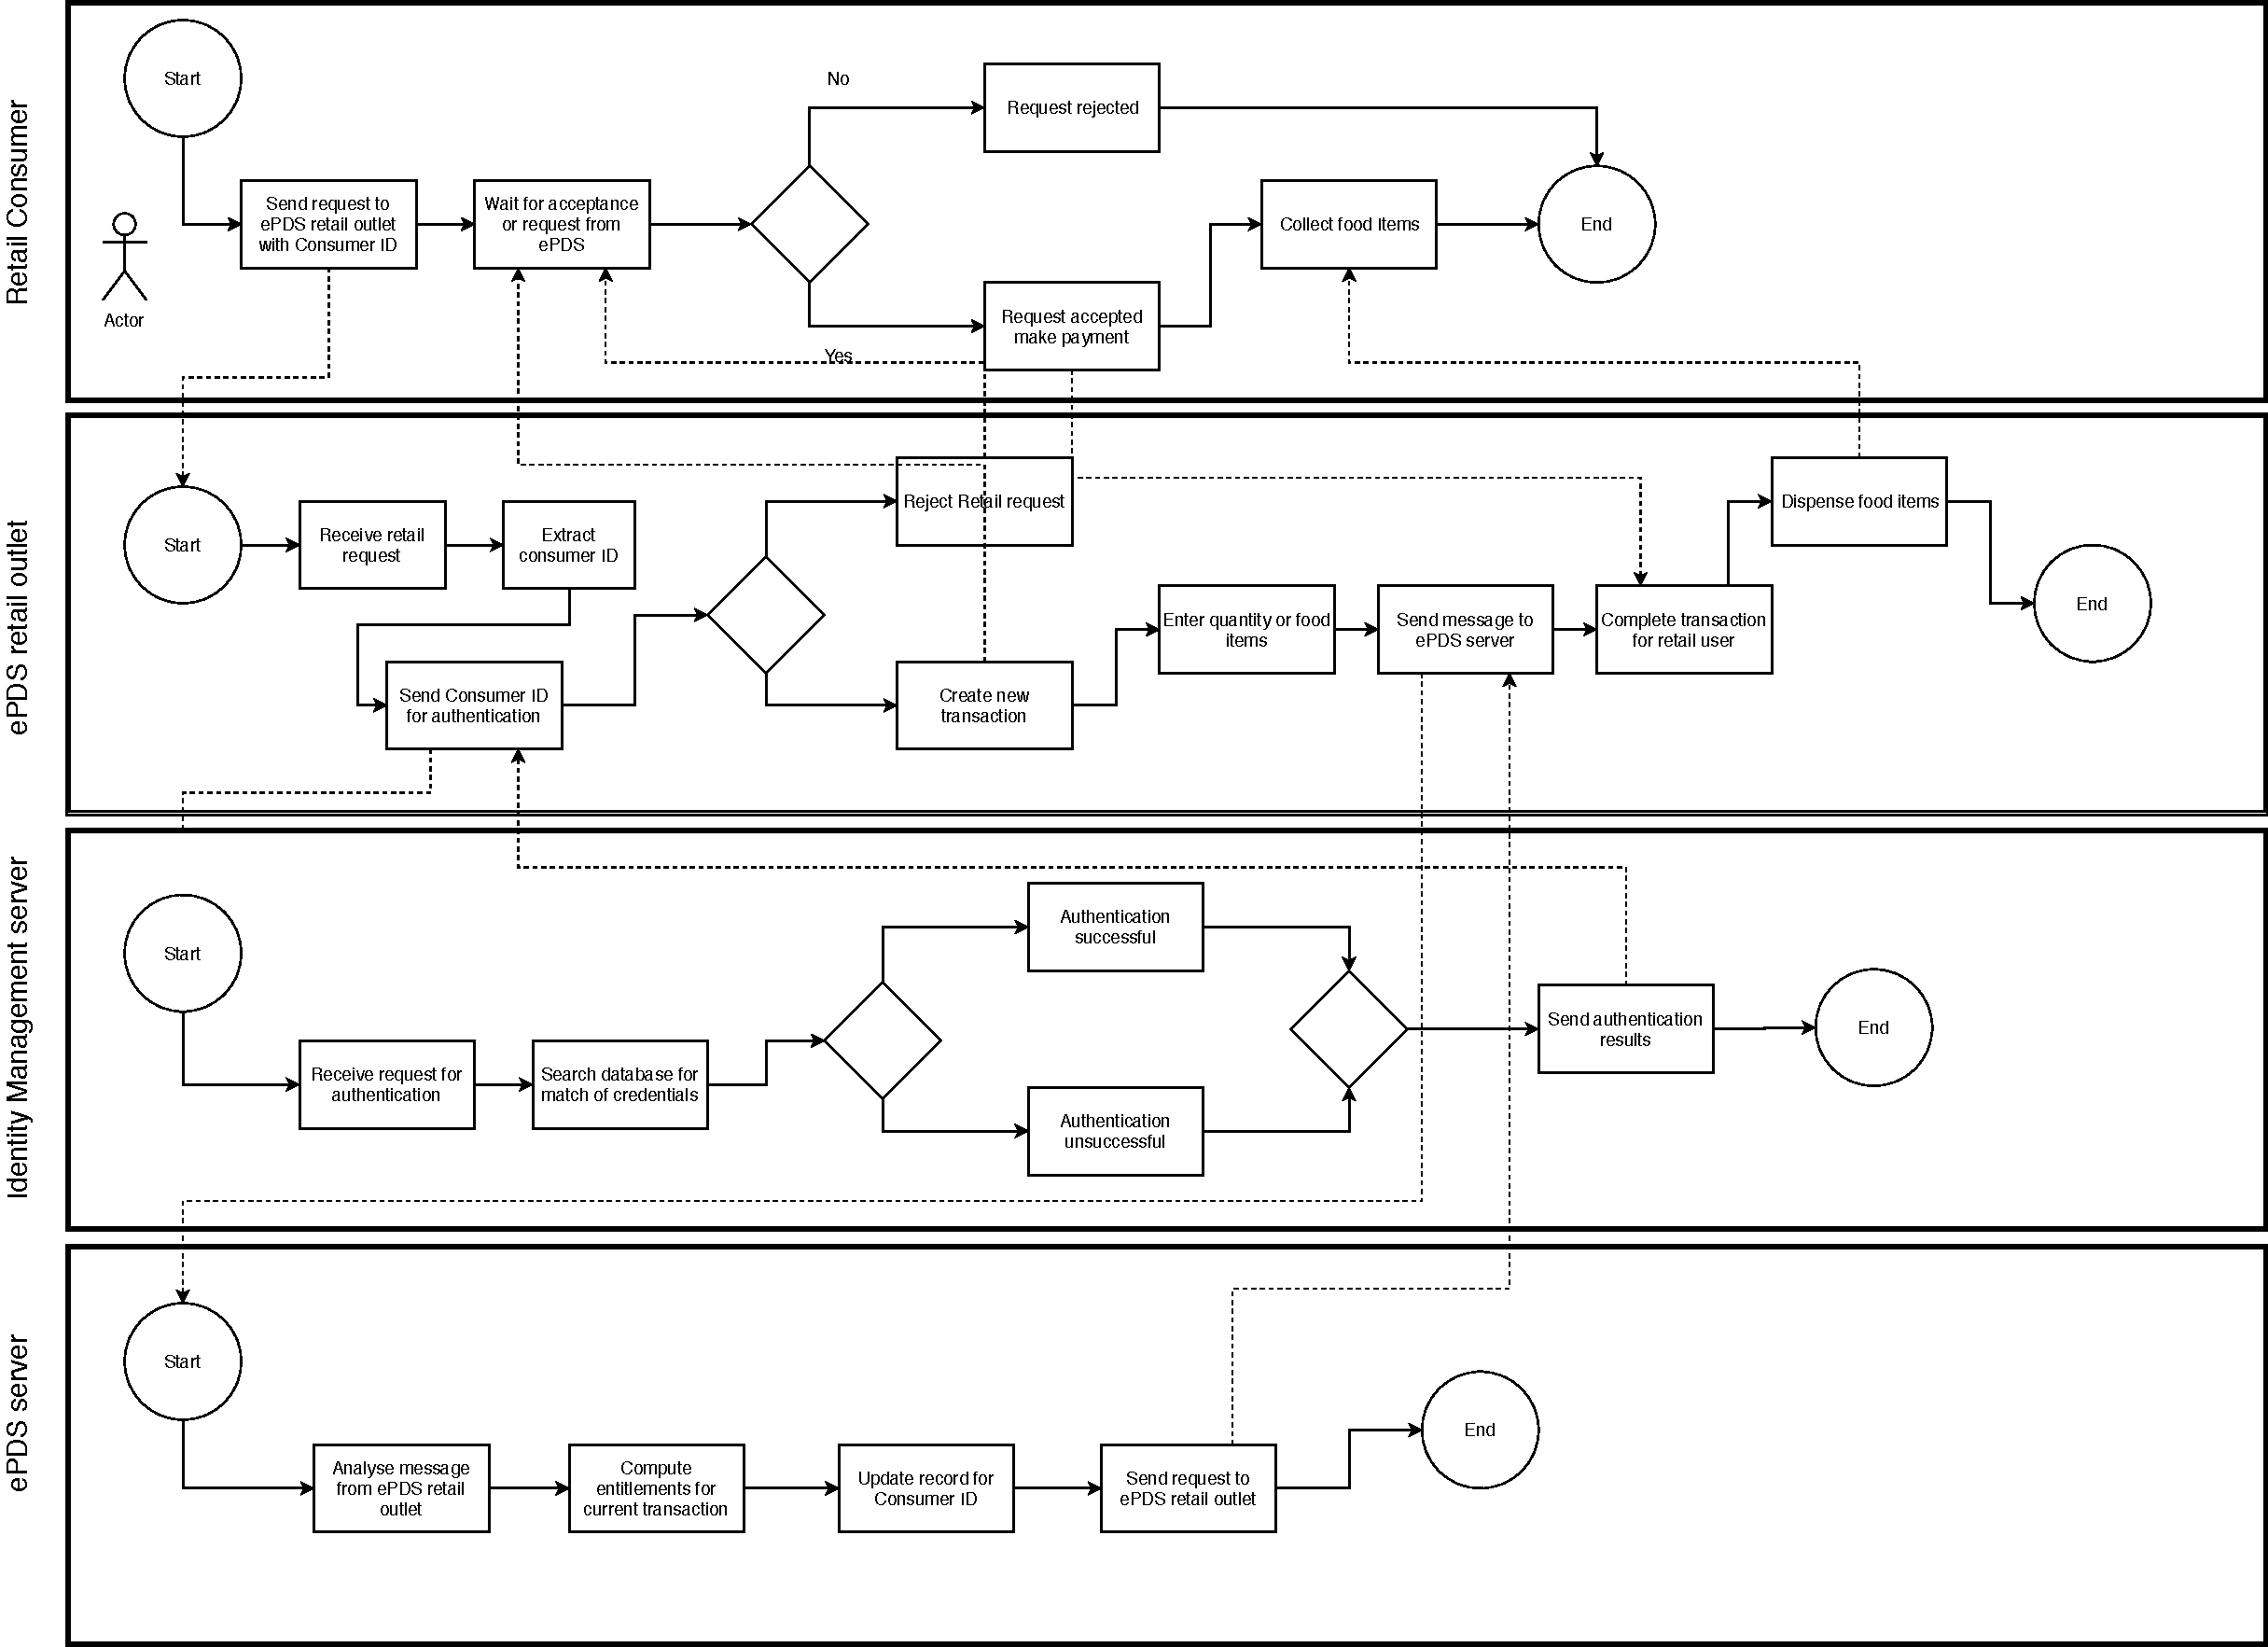
\includegraphics[width=20cm]{epds-functional-diagram}
\captionof{figure}{Proposed functional description of the model}
\end{figure}
\end{landscape}

We have divided the model into four major portions: retail consumer, ePDS retail ouput, identity management sector and ePDS server. When a retail consumer makes a request, the consumer's digital identity is sent by the retail outlet to the centralized identity management service to authenticate the consumer in real time. On successful authentication of the consumer's identity, a request is sent to the SmartPDS backend server for the food entitlements that are to be provided to the targeted consumer. On receiving the list of food entitlements, the retail outlet collects payment and dispenses the requested food items. Since the back-end server maintains a record of all transactions, it provides a check on the retail service provider and helps improve transparency in the distribution system.


\subsection{Advantages}

Improvement in service delivery is achieved through the use of electronic forms on low-cost cell-phones under the supervision of a workflow system to manage requests from mobile users and generate SMS alerts when the goods are ready. \\ \\Improvement in transparency is achieved through the tracking mechanism of a service request from its initiation by the consumer to its fulfillment by the retail outlet. Similarly, the transfer of entitlement benefits to the intended consumers is achieved through the use of electronic vouchers managed by a workflow-based tracking system. \\ \\ Transfer of benefits through an eVoucher system ensures cashless delivery which improves compliance for the targeted consumers. \\ \\This also helps in empowering poor consumers to access these food entitlement services at their doorstep.


\section{Conclusions}

This document presents a mobile technology enabled solution for improving service delivery in the Public Distribution System in India. Since the ePDS system uses mobile connectivity to properly authenticate users in a central database for transactions between the retail outlet and the end consumer, exclusion and inclusion errors can be controlled in near real-time. The mobile phone based ePDS system is scalable and replicable since it uses low-cost cell-phones and the existing cellular infrastructure. Hence the cost of technology intervention is relatively low and it can be replicated in other developing countries.

\pagebreak

\begin{thebibliography}{99}

\bibitem{c1} Planning Commission : \href{http://planningcommission.nic.in/plans/planrel/fiveyr/10th/volume2/v2_ch3_4.pdf}{website}
\bibitem{c2} \href{http://www.prsindia.org/administrator/uploads/general/1388728622~~TPDS%20Thematic%20Note.pdf}{PRS India}
\bibitem{c3} \href{http://www.kscst.iisc.ernet.in/spp/41_series/40S_bestprojreports/40S_BE_0366.pdf}{KSTS}
\bibitem{c4} \href{https://ac.els-cdn.com/S1877050915003324/1-s2.0-S1877050915003324-main.pdf?_tid=9ac7b378-d73e-435a-8ff6-14051bf3e25c&acdnat=1524581743_16e91753752ba258816d70c10d11c6c3}{Automated Ration Distribution System : Science Direct}
\bibitem{c5} \href{https://geleservices.com/GEL/Download/RFP-POS%20.pdf}{POS Based distribution system : Elsevier}
\bibitem{c6} \href{http://www.epw.in/journal/2017/50/special-articles/aadhaar-and-food-security-jharkhand.html}{Aadhaar and food security in Jharkhand : Economics and Political Weekly}
\bibitem{c7} Khera R, (2011) India's Public Distribution System: Utilisation and Impact. The Journal of Development Studies 47 (7), 1038-1060
\bibitem{c8} \href{http://www.ijsrd.com/articles/IJSRDV4I90439.pdf}{Major Drawbacks of PDS : .Mahalingam, Akash Raj D}


\end{thebibliography}





\end{document}